%%% LaTeX-Vorlage Version 1.8 %%%

% Grundlegende Dokumenteneigenschaften gemäß DHBW-Vorgaben
\documentclass[a4paper,fontsize=11pt,oneside,parskip=half,headings=normal,listof=nochaptergap]{scrreprt} 
% \usepackage{showframe} % nur für Kontrolle der Ränder 

%%% Präambel einbinden (mit Festlegungen gemäß DHBW-Vorgaben) %%%
%%% Präambel %%%
% hier sollten keine Änderungen erforderlich sein
%
\usepackage[utf8]{inputenc}   % Zeichencodierung UTF-8 für Eingabe-Dateien
\usepackage[T1]{fontenc}      % Darstellung von Umlauten im PDF

\usepackage{listings}         % für Einbindung von Code-Listings
\usepackage{xcolor}
\usepackage{booktabs}

\renewcommand\lstlistlistingname{Listingsverzeichnis}

\definecolor{codegreen}{rgb}{0,0.6,0}
\definecolor{codegray}{rgb}{0.5,0.5,0.5}
\definecolor{codepurple}{rgb}{0.58,0,0.82}
\definecolor{backcolour}{rgb}{0.95,0.95,0.92}

\lstdefinestyle{mystyle}{
  backgroundcolor=\color{backcolour},
  commentstyle=\color{codegreen},
  keywordstyle=\color{magenta},
  numberstyle=\tiny\color{codegray},
  stringstyle=\color{codepurple},
  basicstyle=\ttfamily\footnotesize,
  breakatwhitespace=false,
  breaklines=true,
  captionpos=b,
  keepspaces=true,
  numbers=left,
  numbersep=5pt,
  showspaces=false,
  showstringspaces=false,
  showtabs=false,
  tabsize=2,
  numberbychapter=false
}

\lstset{style=mystyle}

\lstset{literate=             % erlaubt Sonderzeichen in Code-Listings 
  {Ö}{{\"O}}1
{Ä}{{\"A}}1
{Ü}{{\"U}}1
{ß}{{\ss}}2
{ü}{{\"u}}1
{ä}{{\"a}}1
{ö}{{\"o}}1
{€}{{\euro}}1
}

\usepackage[
  inner=35mm,outer=15mm,top=25mm,
  bottom=20mm,foot=12mm,includefoot
]{geometry}                 % Einstellungen für Ränder
\usepackage{tabularx}
\usepackage[ngerman]{babel} % Spracheinstellungen Deutsch
\usepackage[babel,german=quotes]{csquotes} % deutsche Anf.zeichen
\usepackage{enumerate}      % anpassbare Nummerier./Aufz.
\usepackage{graphicx}       % Einbinden von Grafiken
\usepackage[onehalfspacing]{setspace} % anderthalbzeilig

\usepackage{blindtext}      % Textgenerierung für Testzwecke
\usepackage{color}          % Verwendung von Farbe 
\usepackage{pgfplots}      % für Diagramme
\pgfplotsset{compat=1.16}
\usepackage{tikz}
\usepackage{graphicx}
\usepackage{listings}
\usepackage{xcolor}
\definecolor{delim}{RGB}{20,105,176}
\definecolor{numb}{RGB}{106, 109, 32}
\definecolor{string}{rgb}{0.64,0.08,0.08}
\definecolor{backcolour}{rgb}{1,1,1}

\lstdefinelanguage{json}{
    basicstyle=\ttfamily\small\color{black},
    backgroundcolor=\color{backcolour},
    numbers=left,
    numberstyle=\small\color{gray},
    stepnumber=1,
    numbersep=8pt,
    showstringspaces=false,
    breaklines=true,
    frame=single,
    literate=
     *{0}{{{\color{numb}0}}}{1}
      {1}{{{\color{numb}1}}}{1}
      {2}{{{\color{numb}2}}}{1}
      {3}{{{\color{numb}3}}}{1}
      {4}{{{\color{numb}4}}}{1}
      {5}{{{\color{numb}5}}}{1}
      {6}{{{\color{numb}6}}}{1}
      {7}{{{\color{numb}7}}}{1}
      {8}{{{\color{numb}8}}}{1}
      {9}{{{\color{numb}9}}}{1}
      {\{}{{{\color{delim}{\{}}}}{1}
      {\}}{{{\color{delim}{\}}}}}{1}
      {[}{{{\color{delim}{[}}}}{1}
      {]}{{{\color{delim}{]}}}}{1}
      {,}{{{\color{delim}{,}}}}{1}
      {:}{{{\color{delim}{:}}}}{1},
    morestring=[b]",
    stringstyle=\color{red},   % Dies färbt alle Strings rot.
}
\usepackage[printonlyused]{acronym}        % für ein Abkürzungsverzeichnis

\usepackage[                % Biblatex
  backend=biber,
  bibstyle=_dhbw_authoryear,maxbibnames=99,
  citestyle=authoryear,
  uniquename=true, useprefix=true,
  bibencoding=utf8]{biblatex}
%kein Punkt am Ende bei \footcite
%http://www.golatex.de/footcite-ohne-punkt-am-schluss-t4865.html
\renewcommand{\bibfootnotewrapper}[1]{\bibsentence#1}


%Reihenfolge der Autorennamen
%   
% http://golatex.de/viewtopic,p,80448.html#80448
% Argumente: siehe http://texwelt.de/blog/modifizieren-eines-biblatex-stils/
\DeclareNameFormat{sortname}{% Bibliographie
  \ifnum\value{uniquename}=0 % Normalfall
  \ifuseprefix%
    {%
    \usebibmacro{name:family-given}
    {\namepartfamily}
    {\namepartgiveni}
    {\namepartprefix}
    {\namepartsuffixi}%
    }
    {%
    \usebibmacro{name:family-given}
    {\namepartfamily}
    {\namepartgiveni}
    {\namepartprefixi}
    {\namepartsuffixi}%
    }%
  \fi
  \ifnum\value{uniquename}=1% falls nicht eindeutig, abgek. Vorname 
    {%
    \usebibmacro{name:family-given}
    {\namepartfamily}
    {\namepartgiveni}
    {\namepartprefix}
    {\namepartsuffix}%
    }%
  \fi
  \ifnum\value{uniquename}=2% falls nicht eindeutig, ganzer Vorname 
    {%
    \usebibmacro{name:family-given}
    {\namepartfamily}
    {\namepartgiven}
    {\namepartprefix}
    {\namepartsuffix}%
    }%
  \fi
  \usebibmacro{name:andothers}}

\DeclareNameFormat{labelname}{% für Zitate
  \ifnum\value{uniquename}=0 % Normalfall
  \ifuseprefix%
    {%
    \usebibmacro{name:family-given}
    {\namepartfamily}
    {\empty}
    {\namepartprefix}
    {\namepartsuffixi}%
    }
    {%
    \usebibmacro{name:family-given}
    {\namepartfamily}
    {\empty}
    {\namepartprefixi}
    {\namepartsuffixi}%
    }%
  \fi
  \ifnum\value{uniquename}=1% falls nicht eindeutig, abgek. Vorname 
    {%
    \usebibmacro{name:family-given}
    {\namepartfamily}
    {\namepartgiveni}
    {\namepartprefix}
    {\namepartsuffix}%
    }%
  \fi
  \ifnum\value{uniquename}=2% falls nicht eindeutig, ganzer Vorname 
    {%
    \usebibmacro{name:family-given}
    {\namepartfamily}
    {\namepartgiven}
    {\namepartprefix}
    {\namepartsuffix}%
    }%
  \fi
  \usebibmacro{name:andothers}}


\DeclareFieldFormat{extrayear}{% = the 'a' in 'Jones 1995a'
  \iffieldnums{labelyear}
  {\mknumalph{#1}}
  {\mknumalph{#1}}}

\renewcommand*{\multinamedelim}{\addslash}
\renewcommand*{\finalnamedelim}{\addslash}
\renewcommand*{\multilistdelim}{\addslash}
\renewcommand*{\finallistdelim}{\addslash}

\renewcommand{\nameyeardelim}{~}

% Literaturverzeichnis: Doppelpunkt zwischen Name (Jahr): Rest 
% http://de.comp.text.tex.narkive.com/Tn1HUIXB/biblatex-authoryear-und-doppelpunkt
\renewcommand{\labelnamepunct}{\addcolon\addspace}

% damit die Darstellung für Vollzitate von Primärquellen in 
% Fußnoten später auf "nicht fett" geändert werden kann 
% (nur für Zitate von Sekundärliteratur relevant)
\newcommand{\textfett}[1]{\textbf{#1}}

% für Zitate von Sekundärliteratur:
\newcommand{\footcitePrimaerSekundaer}[4]{%
  \renewcommand{\textfett}[1]{##1}%
  \footnote{\fullcite[#2]{#1}, zitiert nach \cite[#4]{#3}}%  
  \renewcommand{\textfett}[1]{\textbf{##1}}%
}

% Im Literaturverzeichnis: Autor (Jahr) fett
\renewbibmacro*{author}{%
  \ifboolexpr{%
    test \ifuseauthor%
    and
    not test {\ifnameundef{author}}
  }
  {\usebibmacro{bbx:dashcheck}
    {\bibnamedash}
    {\usebibmacro{bbx:savehash}%
      \textfett{\printnames{author}}%
      \iffieldundef{authortype}
      {\setunit{\addspace}}
      {\setunit{\addcomma\space}}}%
    \iffieldundef{authortype}
    {}
    {\usebibmacro{authorstrg}%
      \setunit{\addspace}}}%
  {\global\undef\bbx@lasthash
    \usebibmacro{labeltitle}%
    \setunit*{\addspace}}%
  \textfett{\usebibmacro{date+extrayear}}}

% Sonderfall: Quelle ohne Autor, aber mit Herausgeber
% Name des Herausgebers wird fett gedruckt
\renewbibmacro*{bbx:editor}[1]{%
  \ifboolexpr{%
    test \ifuseeditor%
    and
    not test {\ifnameundef{editor}}
  }
  {\usebibmacro{bbx:dashcheck}
    {\bibnamedash}
    {\textfett{\printnames{editor}}%
      \setunit{\addcomma\space}%
      \usebibmacro{bbx:savehash}}%
    \usebibmacro{#1}%
    \clearname{editor}%
    \setunit{\addspace}}%
  {\global\undef\bbx@lasthash
    \usebibmacro{labeltitle}%
    \setunit*{\addspace}}%
  \textfett{\usebibmacro{date+extrayear}}}

% Anpassungen für deutsche Sprache
\DefineBibliographyStrings{ngerman}{%
  nodate = {{o.J.}},
  urlseen = {{Abruf:}},
  ibidem = {{ebenda}}
}

% keine Anführungszeichen beim Titel im Literaturverzeichnis
\DeclareFieldFormat[article,book,inbook,inproceedings,manual,misc,phdthesis,thesis,online,report]{title}{#1\isdot}

\newcommand{\literaturverzeichnis}{%
  % nur Literaturverzeichnis
  % (als eigenes Kapitel)
  \phantomsection
  \addcontentsline{toc}{chapter}{Literaturverzeichnis}
  \spezialkopfzeile{Literaturverzeichnis}
  \defbibheading{lit}{\chapter*{Literaturverzeichnis}}
  \label{chapter:quellen}
  \printbibliography[heading=lit,notkeyword=ausblenden]
} % mit DHBW-spezifischen Einstellungen

\usepackage[hidelinks]{hyperref}       % URL-Formatierung, klickbare Verweise

\usepackage{tocloft}        % für Verzeichnis der Anhänge


\newcounter{anhcnt}
\setcounter{anhcnt}{0}
\newlistof{anhang}{app}{}

\newcommand{\anhang}[1]{%
  \refstepcounter{anhcnt}
  \setcounter{anhteilcnt}{0}
  \section*{Anhang \theanhcnt: #1}
  \addcontentsline{app}{section}{\protect\numberline{Anhang \theanhcnt}#1}\par
}

\newcounter{anhteilcnt}
\setcounter{anhteilcnt}{0}

\newcommand{\anhangteil}[1]{%
  \refstepcounter{anhteilcnt}
  \subsection*{Anhang~\arabic{anhcnt}/\arabic{anhteilcnt}: #1}
  \addcontentsline{app}{subsection}{\protect\numberline{Anhang \theanhcnt/\arabic{anhteilcnt}}#1}\par
}

\renewcommand{\theanhteilcnt}{Anhang \theanhcnt/\arabic{anhteilcnt}}

% vgl. S. 4 Paket-Beschreibung tocloft 	
% Einrückungen für Anhangverzeichnis
\makeatletter
\newcommand{\abstaendeanhangverzeichnis}{
  \renewcommand*{\l@section}{\@dottedtocline{1}{0em}{5.5em}}
  \renewcommand*{\l@subsection}{\@dottedtocline{2}{2.3em}{6.5em}}
}
\makeatother

% Abbildungs- und Tabellenverzeichnis
% Bezeichnungen
\renewcaptionname{ngerman}{\figurename}{Abb.}
\renewcaptionname{ngerman}{\tablename}{Tab.}
% Einrückungen
\makeatletter
\renewcommand*{\l@figure}{\@dottedtocline{1}{0em}{2.3em}}
\renewcommand*{\l@table}{\@dottedtocline{1}{0em}{2.3em}}
\makeatother


\usepackage{chngcntr}                % fortlaufende Zähler für Fußnoten, Abbildungen und Tabellen
\counterwithout{figure}{chapter}
\counterwithout{table}{chapter}
\counterwithout{footnote}{chapter}

\usepackage[automark]{scrlayer-scrpage}
%% Definitionen für Kopf- und Fußzeile auf normalen Seiten
\defpagestyle{kopfzeile}
{% Kopfdefinition
  (\textwidth,0pt)    % Länge der oberen Linie,Dicke der oberen Linie       
  {} % Definition für linke Seiten im doppelseitigen Layout
    {} % Definition für rechte Seiten im doppelseitigen Layout      
    {  % Definition für Seiten im einseitigen Layout
      \makebox[0pt][l]{\rightmark}% 
      \makebox[\linewidth]{}% 
    }
  (\textwidth, 0.4pt) % Untere Linienlänge, Untere Liniendicke
}
{% Fußdefinition
  (\textwidth,0pt)    % Obere Linienlänge, Obere Liniendicke
  {} % Definition für linke Seiten im doppelseitigen Layout
    {} % Definition für rechte Seiten im doppelseitigen Layout
    {  % Definition für Seiten im einseitigen Layout
      \makebox[\linewidth]{}%
      \makebox[0pt][r]{\pagemark}%
    }
  (\textwidth, 0pt)   % Länge der unteren Linie,Dicke der unteren Linie
}

%% Definitionen für Kopf- und Fußzeile auf ersten Seiten eines Kapitels
\defpagestyle{kapitelkopfzeile}
{% Kopfdefinition
  (\textwidth,0pt)    % Länge der oberen Linie,Dicke der oberen Linie       
  {} % Definition für linke Seiten im doppelseitigen Layout
    {} % Definition für rechte Seiten im doppelseitigen Layout      
    {}  % Definition für Seiten im einseitigen Layout
  (\textwidth, 0pt) % Untere Linienlänge, Untere Liniendicke
}
{% Fußdefinition
  (\textwidth,0pt)    % Obere Linienlänge, Obere Liniendicke
  {} % Definition für linke Seiten im doppelseitigen Layout
    {} % Definition für rechte Seiten im doppelseitigen Layout
    {  % Definition für Seiten im einseitigen Layout
      \makebox[\linewidth]{}%
      \makebox[0pt][r]{\pagemark}%
    }
  (\textwidth, 0pt)   % Länge der unteren Linie,Dicke der unteren Linie
}

%% Definitionen für Kopf- und Fußzeile im Anhang und bei Quellenverzeichnisse
\newcommand{\spezialkopfzeileBezeichnung}{}
\defpagestyle{spezialkopfzeile}
{% Kopfdefinition
  (\textwidth,0pt)    % Länge der oberen Linie,Dicke der oberen Linie       
  {} % Definition für linke Seiten im doppelseitigen Layout
    {} % Definition für rechte Seiten im doppelseitigen Layout      
    {  % Definition für Seiten im einseitigen Layout
      \makebox[0pt][l]{\spezialkopfzeileBezeichnung}% 
      \makebox[\linewidth]{}% 
    }
  (\textwidth, 0.4pt) % Untere Linienlänge, Untere Liniendicke
}
{% Fußdefinition
  (\textwidth,0pt)    % Obere Linienlänge, Obere Liniendicke
  {} % Definition für linke Seiten im doppelseitigen Layout
    {} % Definition für rechte Seiten im doppelseitigen Layout
    {  % Definition für Seiten im einseitigen Layout
      \makebox[\linewidth]{}%
      \makebox[0pt][r]{\pagemark}%
    }
  (\textwidth, 0pt)   % Länge der unteren Linie,Dicke der unteren Linie
}

\newcommand\spezialkopfzeile[1]{%
  \renewcommand\spezialkopfzeileBezeichnung{#1}
  \pagestyle{spezialkopfzeile}
}

% Standard-Pagestyle auswählen
\pagestyle{kopfzeile}

% keine Kopfzeile anzeigen auf Seiten, auf denen ein 
% Kapitel beginnt oder das Inhalts-/Abbildungs-/Tabellenverzeichnis steht 
\renewcommand{\chapterpagestyle}{kapitelkopfzeile}
\tocloftpagestyle{kapitelkopfzeile}

		 % für schöne Kopfzeilen 

\usepackage{textcomp}            % erlaubt EUR-Zeichen in Eingabedatei
\usepackage{eurosym}             % offizielles EUR-Symbol in Ausgabe
\renewcommand{\texteuro}{\euro}  % ACHTUNG: nach hyperref aufrufen!

\usepackage{scrhack}             % stellt Kompatibilität zw. KOMA-Script
% (scrreprt) und anderen Paketen her

% Anpassung der Abstände bei Kapitelüberschriften
% (betrifft auch Inhalts-, Abbildungs- und Tabellenverzeichnis)
\renewcommand*\chapterheadstartvskip{\vspace*{-\topskip}}
\newcommand{\myBeforeTitleSkip}{1mm}
\newcommand{\myAfterTitleSkip}{10mm}
\setlength\cftbeforetoctitleskip{\myBeforeTitleSkip}
\setlength\cftbeforeloftitleskip{\myBeforeTitleSkip}
\setlength\cftbeforelottitleskip{\myBeforeTitleSkip}

\setlength\cftaftertoctitleskip{\myAfterTitleSkip}
\setlength\cftafterloftitleskip{\myAfterTitleSkip}
\setlength\cftafterlottitleskip{\myAfterTitleSkip}
%%% Ende der Präambel %%%


%%% Name der eigenen Literatur-Datenbank (ggf. anpassen) %%%
\bibliography{includes/literatur.bib}

\begin{document}
%%% Deckblatt einbinden %%% 
% Anpassungen nötig (Name, Titel etc.)
% HIER EDITIEREN: 
% Typ der Arbeit (für Deckblatt und Metadaten)
% - bitte Zutreffendes auswählen
%\newcommand{\typMeinerArbeit}{1. Projektarbeit}
%\newcommand{\typMeinerArbeit}{2. Projektarbeit}
%\newcommand{\typMeinerArbeit}{Seminararbeit}
\newcommand{\typMeinerArbeit}{Bachelorarbeit}

% Thema der Arbeit (für ehrenwörtliche Erklärung, ohne Umbrüche)
% HIER EDITIEREN: 
\newcommand{\themaMeinerArbeit}{Document Understanding Transformers in der Dokumentenverarbeitung}

% Vorname, Name der Autorin/des Autors (für Titelseite und Metadaten)
% HIER EDITIEREN:
\newcommand{\meinName}{Marc Novak}

\thispagestyle{empty}

\begin{spacing}{1}
  \begin{center}
    ~\vspace{0mm}

    % HIER EDITIEREN: Titel der Arbeit
    {\sffamily
      \LARGE
      % \Large  % bei sehr langen Titeln ggf. etwas kleinere Schriftart wählen
      \textbf{Document Understanding Transformers in der Dokumentenverarbeitung}

      \bigskip
      \textbf{}
    }


    \vspace{15mm}

    % Typ wird automatisch eingefügt (oben festlegen)
    {\Large \typMeinerArbeit}

    \vspace{1cm}

    % HIER ggf. EDITIEREN
    vorgelegt am \today

    \vspace{15mm}

    Fakultät Wirtschaft
    \medskip

    Studiengang Wirtschaftsinformatik
    \medskip

    % HIER EDITIEREN: Kurs eintragen
    Kurs WI2021G

    \vspace{10mm}

    von

    \vspace{10mm}

    % Vorname und Name wird automatisch eingefügt (oben festlegen) 
    {\large\textsc{\meinName}}

    \vspace{10mm}
  \end{center}

  \vfill

  % HIER EDITIEREN: Name des Unternehmens, Name der Betreuerin/des Betreuers
  \begin{tabular}{ll}
    Betreuer in der Ausbildungsstätte:        & DHBW Stuttgart:                                                    \\
    \hspace{0.4\linewidth}                    &                                                                    \\
    ELO Digital Office GmbH & $\langle$ Titel, Vorname und Nachname $\rangle$                    \\
    Dr. Konstantin Hauch
                                              & $\langle$ der/des wissenschaftlichen Betreuerin/Prüferin $\rangle$ \\
    Teamleiter Team KI                                                     \\
    \\
    Unterschrift der Betreuerin/des Betreuers                                                                      \\
  \end{tabular}


  \vspace{1cm}
  %(etwas Platz für die Unterschrift der Betreuerin/des Betreuers aus der Ausbildungsstätte)
\end{spacing}

% falls ein Vertraulichkeitsvermerk erforderlich ist,
% die Kommentarzeichen in den nachfolgenden Zeilen entfernen:

%\begin{center}
%\small
%\textbf{Vertraulichkeitsvermerk}:
%Der Inhalt dieser Arbeit darf weder als Ganzes noch in Auszügen \\
%Personen außerhalb des Prüfungs- und Evaluationsverfahrens zugänglich gemacht werden, sofern keine anders lautende Genehmigung des Dualen Partners vorliegt. 
%\end{center}

% Meta-Daten für PDF-Datei basierend auf obigen Angaben
\hypersetup{pdftitle={\themaMeinerArbeit}}
\hypersetup{pdfauthor={\meinName}}
\hypersetup{pdfsubject={\typMeinerArbeit\ DHBW Stuttgart \the\year}}


%%% Umstellung der Seiten-Nummerierung auf i, ii, iii ... %%%
\pagenumbering{Roman}
\cleardoublepage

%%% Inhalts-, Abbildungs-, Tabellenverzeichnisse %%%
% sollen einzeilig gesetzt werden, um Platz zu sparen 
\begin{spacing}{1}
  \tableofcontents
  \clearpage
  \chapter*{Abkürzungsverzeichnis}
\addcontentsline{toc}{chapter}{Abkürzungsverzeichnis}

\begin{acronym}[DHBW]
  % Argument definiert die Breite der ersten Spalte anhand des längsten vorkommenden Eintrags
  \acro{CRM}{Customer Relationship Management}
  \acro{DHBW}{Duale Hochschule Baden-Württemberg}
  \acro{IEEE}{Institute of Electrical and Electronics Engineers}
  \acro{ITIL}{IT Infrastructure Library}
  \acro{RoI}{Return-On-Invest}
  \acro{UCS}{Universal Character Set}
  \acro{UTF-8}{8-Bit UCS Transformation Format}
\end{acronym}

\vspace{2em}


  \clearpage
  \thispagestyle{kapitelkopfzeile}
  \listoffigures
  \phantomsection
  \addcontentsline{toc}{chapter}{Abbildungsverzeichnis} % Abb.verz. ins Inh.verz. aufnehmen

  \clearpage
  \listoftables
  \phantomsection
  \addcontentsline{toc}{chapter}{Tabellenverzeichnis}   % Tab.verz. ins Inh.verz. aufnehmen
  \clearpage
  \lstlistoflistings
  \addcontentsline{toc}{chapter}{Listingsverzeichnis}   % Lst.verz. ins Inh.verz. aufnehmen
\end{spacing}

%%% Umstellung der Seiten-Nummerierung auf 1, 2, 3 ... %%%
\cleardoublepage
\pagenumbering{arabic}

%%% Ihr eigentlicher Inhalt %%%
% Empfehlung: strukturieren Sie Ihren Text in einzelnen Dateien 
% und binden Sie diese hier mit \input{includes/dateiname.tex} ein
\chapter{Einleitung}

In den vergrangenen Jahren hat \ac{KI} in Unternehmen zunehmend an Bedeutung gewonnen. Seit 2019 verzeichnet der KI-Software Markt einen hohes Wachstum. Es wird davon ausgegangen, dass dieses Wachstum bis 2025 mit über 26 \% pro Jahr anhalten wird. \footcites[Vgl.][]{howarth_57_2024} Die Anwendungsbereiche von KI-Systemen sind vielfältig und reichen von der Automatisierung von Prozessen, über die Analyse von großen Datenmengen bis hin zur Vorhersage von zukünftigen Ereignissen.

Einer der beliebtesten Anwendungsbereiche von KI-Systemen ist die Dokumentenverarbeitung. Eine Befragung von 1420 IT-Fachkräften ergab, dass 28 \% der zugehörigen Unternehmen KI-Systeme zur Dokumentenverarbeitung einsetzen (s. Abb. \ref{fig:ai_tech_distribution}). \footcites[Vgl.][]{rackspace_most_2023} Die Dokumentenverarbeitung umfasst die Extraktion von Informationen, die Klassifizierung und die automatisierte Verarbeitung von Dokumenten.\footcites[Vgl.][S.1]{esposito_intelligent_2005} Die Verarbeitung von Dokumenten ist in vielen Unternehmen ein zeitaufwändiger Prozess, der durch den Einsatz von KI-Systemen automatisiert und beschleunigt werden kann.\footcites[Vgl.][S.11]{dutt_now_2024}

\pgfplotsset{compat=1.17} % Use the version of pgfplots you have installed

\begin{figure}[htb]
    \centering
\begin{tikzpicture}
    \begin{axis}[
        xbar, % Horizontal bars
        xmin=0, xmax=60, % Set the minimum and maximum x-coordinates
        width=11cm, height=9cm, % Width and height of the plot
        enlarge y limits=0.1, % Add some space between bars
        xlabel={Share of respondents in \%}, % Label for the x-axis
        symbolic y coords={
            Speech recognition,
            Image recognition,
            Facial recognition,
            Sales and marketing analytics,
            Document processing,
            Intelligent search,
            Recommender systems,
            Natural language processing,
            Predictive maintenance,
            Customer engagement,
            Computer vision
        },
        ytick=data, % Use the data for y-ticks
        nodes near coords,
        nodes near coords align={anchor=west}, % Add the percentage labels near the bars% Align the labels horizontally
        point meta=explicit symbolic % The meta data is explicitly given as symbolic text
    ]
    \addplot [draw=blue,fill=blue!30 ] coordinates {
        (51,Computer vision)[51\%]
        (47,Customer engagement)[47\%]
        (43,Predictive maintenance)[43\%]
        (38,Natural language processing)[38\%]
        (34,Recommender systems)[34\%]
        (31,Intelligent search)[31\%]
        (28,Document processing)[28\%]
        (26,Sales and marketing analytics)[26\%]
        (23,Facial recognition)[23\%]
        (18,Image recognition)[18\%]
        (13,Speech recognition)[13\%]};
    \end{axis}
\end{tikzpicture}
\caption[Gängigste Verwendungszwecke von KI in Unternehmen]{Gängigsten Verwendungszwecke von KI in Unternehmen\footnotemark} % Caption for the figure
    \label{fig:ai_tech_distribution} % Label for referencing the figure
\end{figure}
\footnotetext{Entnommen aus: \cite{rackspace_most_2023}}

Die Verarbeitung von gescannten Dokumenten, insbesondere von Rechnungen ist ein integraler Bestandteil der Dokumentenverarbeitung. Der Einsatz von \ac{OCR} ermöglicht die Digitalisierung und elektronische Weiterverarbeitung dieser Dokumente. Jeoch ist die Zuordnung der erkannten Zeichenketten zu interpretierbaren Metadaten oft von manueller Nachbearbeitung oder von regulären Ausdrücken abhängig. Eine weitere Hürde, welche sich bei der Extraktion von Informationen aus Rechnungen zeigt, sind die sehr heterogenen Vorlagen und Layouts, welche in der Verarbeitung zu Ungenauigkeiten führen kann. Die OCR kann hier nicht mehr sicher die erkannten Werte den entsprechenden Labeln zuordnen.\footcites[Vgl.][S.1]{rahal_information_2018} Die DMS-Software \ac{ELO} von ELO verarbeitet Rechnungen zurzeit mittels OCR. Die Anwendung von Transformer-Modellen, im Bereich des \ac{VDU} ermöglicht eine direkte kontextbasierte Weiterverarbeitung der Rechnungen.\footcites[Vgl.][S.1]{kim_ocr-free_2021}

Diese Arbeit untersucht neue Transformer-Modelle im Bereich des VDU. Es wird analysiert, wie diese Modelle, die ihren Ursprng in der natürlichen Sprachverarbeitung haben, auf die Interpretation visueller (layoutbasierter) und textueller Elemente in Dokumenten angewandt werden können. Weiterhin wird ein OCR-freier \ac{Donut} untersucht, um die Limitierungen von OCR bezüglich Laufzeit und Fehleranfälligkeit zu überwinden.\footcites[Vgl.][S.1]{kim_ocr-free_2021} Diese Arbeit umfasst die Bereitstellung einer Pipeline, welche vom Modelltraining des Donuts bis zur Endanwendung im Unternehmen ELO Digital Office GmbH reicht. 
Das Ziel dieser Arbeit ist es, die Anwendbarkeit von Transformer-Modellen im Bereich des \ac{VDU} zu untersuchen und die Leistungsfähigkeit der Pipeline zu evaluieren um folgende Forschungsfrage zu beantworten:
\begin{center}
    \emph{Kann die Anwendung von Document Understanding Transformer Modellen die Effizienz und Genauigkeit der Rechnungsverarbeitung im Vergleich zu bestehenden OCR-basierten Modellen steigern?}
\end{center} 
Um diese Frage zu beantworten wird anhand eines Benchmarks (detaillierte Beschreibung des Aufbaus folgt in Kapitel 3) die Leistungsfähigkeit der Donut-basierten Pipeline mittels diverser Metriken bemessen und zur Leistungsfähigkeit von OCR-basierten Modellen verglichen. Daher ist die Arbeit folgedermaßen strukturiert: \\Zunächst werden in Kapitel 2 die Grundlagen der Dokumentenverarbeitung und der Transformer-Modelle erläutert. In Kapitel 3 werden die zu untersuchenden Modelle ausgewählt. Des weiteren werden der experimentelle Ansatz und der Aufbau der Testumgebung und Datensätze beschrieben. In Kapitel 4 wird die Entwicklung der Pipeline und die Implementierung des Donut dargestellt. Kapitel 5 präsentiert die Ergebnisse des Experiments. Kapitel 6 diskutiert die Ergebnisse und zieht Schlussfolgerungen. Eine Zusammenfassung und ein Ausblick auf zukünftige Arbeiten schließen die Arbeit in Kapitel 7 ab. Mit dieser Strukturierung als Ausgangspunkt, folgt nun die detaillierte Betrachtung der Grundlagen der Dokumentenverarbeitung und der Transformer-Modelle in Kapitel 2.

\chapter{Theoretischer Hintergrund}
Im folgenden Kapitel werden die theoretischen Grundlagen für diese Arbeit erläutert, um ein Verständnis für die verwendeten Begriffe und Technologien zu schaffen. Zunächst wird ein kurzer Überblick über die \ac{OCR} gegeben. Anschließend werden die Grundlagen der Transformer-Modelle erläutert. Des Weiteren werden die Details des \ac{Donut} genauer betrachtet, um ein Verständnis für die Funktionsweise des Modells im Vergleich zu herkömmlichen Methoden zu schaffen.

\section{Grundlagen der OCR}
Dieser Abschnitt betrachtet die grundlegende Funktionsweise und die Anwendungsbereiche von OCR-Systemen, da auch heute noch die meisten Modelle der Dokumentenverarbeitung auf eine OCR für den textuellen Input angewiesen sind (siehe dazu bspw. LayoutLM3\footcites[Vgl. dazu ausführlich][]{huang_layoutlmv3_2022}, ERNIE\footcites[Vgl. dazu ausführlich][]{peng_ernie-layout_2022}, FastStrucText\footcites[Vgl. dazu ausführlich][]{zhai_fast-structext_2023} etc.). Der Abschnitt bietet einen grundlegenden Überblick über das Thema. Auf ein tieferes Verständnis und eine detaillierte Betrachtung der Funktionsweise von OCR-Systemen wird in dieser Arbeit nicht eingegangen, da der Fokus auf der Anwendung von Transformer-Modellen im Bereich der Dokumentenverarbeitung liegt. Dennoch darf die Relevanz von OCR-Systemen nicht unterschätzt werden, da sie in vielen \ac{SOTA}-Modellen immer noch als Basis für die Textextraktion dienen. 

Häufig liegen Informationen in handschriftlicher oder gedruckter Form vor. Diese Informationen können durch Scans als Bilder in Computern gespeichert werden, jedoch ist die weiterverarbeitung der Informationen schwierig. Das System kann nicht ohne weiteres auf den Text in den erfassten Bildern zugreifen, bzw. diesen Lesen. Das Ziel von OCR ist es, Text aus Bildern zu extrahieren. OCR-Systeme sind in der Lage, Text aus gescannten Dokumenten, Fotos oder anderen Bildern zu extrahieren und in maschinenlesbaren Text umzuwandeln. In einem solchen Format können die Informationen weiterverarbeitet und analysiert werden. Somit ermöglicht es OCR einer Maschine, Texte automatisch zu erkennen.\footcites[Vgl.][S.244]{hamad_detailed_2016}

Für eine hohe Qualität und Genauigkeit der Zeichenerkennung erwarten OCR-Systeme eine hohe Qualität der Eingabebilder. Die Qualität der Eingabebilder ist ein entscheidender Punkt für die Genauigkeit der Zeichenerkennung. Einige Faktoren stellen Herausforderungen für die OCR dar, darunter die Szenenkomplexität, ungleiche Beleuchtungsbedingungen, Verzerrungen, Unschärfe und Abbau, Aspektverhältnisse, die Kippung, die Schriftart und mehrsprachige Umgebungen.\footcites[Vgl.][S.245]{hamad_detailed_2016} Die Herausforderungen erfordern fortgeschrittene Algorithmen und Techniken, einschließlich maschinellem Lernen und künstlicher Intelligenz, um die Erkennungsrate zu verbessern. Diese Herausforderungen versucht das Donut-Modell zu überwinden, indem es auf Transformer-Modellen basiert und somit die Limitierungen von OCR-Systemen umgeht.\footcites[Vgl.][S.1]{kim_ocr-free_2021} Um die Ergebnisse von OCR-Systemen zu verbessern werden in der Literatur verschiedene Ansätze vorgeschlagen. Nguyen et. al. schlagen die Verwendung von BERT vor. Als kontextbasiertes Sprachmodell kann BERT die Genauigkeit der OCR-Systeme verbessern, indem es die Kontextinformationen der Wörter berücksichtigt. Die Autoren zeigen, dass BERT die Genauigkeit der OCR-Systeme durch Fehlererkennung und Korrektur verbessern kann.\footcites[Vgl.][S.335 f.]{nguyen_neural_2020} BERT und seine Derivate werden noch heute in vielen \ac{SOTA}-Modellen für die Textextraktion verwendet.\footcites[Vgl. dazu ausführlich][S.4084 ff.]{huang_layoutlmv3_2022} \footcites[Vgl. dazu ausführlich][S.2 ff.]{garncarek_lambert_2020}

Die Funktionsweise von OCR-Systemen kann in sechs Phasen unterteilt werden. Diese Phasen umfassen die Vorverarbeitung, die Segmentierung, die Normalisierung, die Merkmalsextraktion, die Klassifikation und die Postverarbeitung. Das Ziel der Vorverarbeitung ist es, das Eingabebild zu verbessern und zu bereinigen. Die Segmentierung ist der Prozess, bei dem das Bild in einzelne Zeichen oder Wörter aufgeteilt und vom Hintergrund des Bildes getrennt wird. Sie stellt die kritische und maßgebliche Komponente eines OCR-Systems dar. Die Normalisierung ist der Prozess, bei dem die Segmentierungsergebnisse in eine standardisierte Form gebracht werden. In der Merkmalsextraktionsphase extrahiert das System relevante Merkmale von Objekten oder Alphabeten und wandelt diese zu Merkmalsvektoren um. In der Klassifikationsphase werden die Eingaben unterschiedlichen Klassen zugeordnet.\footcites[Vgl.][S.244]{hamad_detailed_2016} Beispielsweise wird in der Klassifikationsphase die Rechnungsnummer einer Klasse \emph{Invoice-Nr.} zugeordnet und das Datum der Klasse \emph{Date}. Es gibt diverse Werkzeuge, um die Klassifikation durchzuführen. Laut Dongre u.a. ist das \emph{Character Classification Problem} verwandt mit der heuristischen Logik, da Menschen Zeichen und Dokumente durch Erfahrung und Lernen erkennen können. Da Neuronale Netze ebenfalls von heuristischer Natur sind, sollten sie sich besonders gut für solche Probleme eignen. \footcites[Vgl.][S.11]{dongre_review_2010} Hier bleibt jedoch unbeachtet, dass die Eignung auch von der Qualität des Netzes selbst abhängt, welche wiederrum von der Qualität der Trainingsdaten abhängig ist.\footcites[Vgl.][S.851]{kavzoglu_increasing_2009} Daher eignet sich das Neuronale Netz als Klassifikator nur dann besonders gut, wenn die Trainingsdaten von hoher Qualität sind und das Netz in der Klassifikation eine hohe Genauigkeit aufweist. In der Postverarbeitung werden abschließend die Klassifikationsergebnisse weiterverarbeitet und korrigiert, um die Genauigkeit des erkannten Textes zu erhöhen.\footcites[Vgl.][S.246 f.]{hamad_detailed_2016} Hier wird das zuvor genannte BERT-Modell eingesetzt, um die Genauigkeit der OCR-Systeme zu verbessern.\footcites[Vgl.][S.335 f.]{nguyen_neural_2020}

Die Anwendungsbereiche der OCR sind vielfältig. Sie reichen von der Digitalisierung von Dokumenten in der Rechtsbranche über die Verarbeitung von Checks in Banken bis ins Gesundheitswesen. Der für diese Arbeit relevante Verwendungszweck ist die Verarbeitung von Rechnungen. OCR-Systeme werden in vielen Organisationen eingesetzt, um Rechnungen zu digitalisieren und diese so zu überwachen.\footcites[Vgl.][S.247 f.]{hamad_detailed_2016}

\section{Transformer-Modelle}
Im Folgenden soll ein Verständnis für die Transformer-Modelle geschaffen werden, welche wiederrum die Grundlage für Donut bilden. Dabei werden zunächst die Herkunft und Relevanz der Transformer-Modelle (folgend auch Transformer genannt) erläutert. Anschließend wird die Funktionsweise der Modelle genauer betrachtet. Dabei werden Schlüsselkonzepte wie die Aufmerksamkeit und das Positional Encoding, sowie die Architektur der Modelle erläutert. Seit der Einführung der Transformer in 2017 durch Vaswani et al. \footcites{vaswani_attention_2017} sind diese zum de facto Standard für eine Reihe verschiedener \ac{NLP} Aufgaben geworden. \ac{NLP} ist ein Teilbereich der Informatik, welcher es ermöglchen soll Computer Sprache auf eine \emph{natürliche} Art und Weise zu verstehen, so wie Menschen. Typischerweise refferenziert dies Aufgaben wie das Verstehen von Gefühlen in Texten, die Spracherkennung und das generieren von Antworten auf Fragen. \footcites[Vgl.][S.1]{beysolow_ii_applied_2018} Mittlerweile werden Transformer in den bekanntesten und meist genutzen Modellen der Welt verwendet, darunter BERT und GPT. \footcites[Vgl.][S. 1]{tunstall_natural_2022} Die beachtliche Leistungsfähigkeit der Transformer zeigt sich in den Benutzerzahlen von ChatGPT (ein ChatBot von OpenAI welcher auf den Transformer-Modellen basiert). Innerhalb von fünf Tage nach der Veröffentlichung des Modells hatte ChatGPT bereits eine Millionen Nutzer. Im Vergleich dazu brauchte Instagram zwei und halb Monate, um die gleiche Anzahl an Nutzern zu erreichen. \footcites[Vgl.][]{buchholz_infographic_2023} Den Status quo, vor der Entwicklung der Transformer, bildeten die \ac{RNN} und \ac{LSTM} Modelle. Transformer erzielen sowohl in der Leistungsfähigkeit als auch in den Trainingskosten bessere Ergebnisse als seine Vorgänger. \footcites[Vgl.][S. 1]{tunstall_natural_2022}

\subsection{Konzepte und Terminologie der Transformer-Modelle}
%TODO: Complete Chapter: Self-Attention, Multi-Head Attention, Positional Encoding, Encoder-Decoder Architektur

\subsection{Encoder-Decoder Architektur}
Das ursprüngliche Transformer-Modell, präsentiert von Vaswani et al. in 2017, basiert auf einer \emph{Encoder-Decoder} Architektur. Diese Architektur eignet sich besonder gut für Situationen, in welchen es sich sowohl bei der Ein- als auch der Ausgabe um Sequenzen handelt. Der Encoder wandelt die Eingabe von einer Sequenz in eine numerische Repräsentation um, welche häufig als \emph{last hidden state} bezeichnet wird. Dieser Zustand wird dann in den Decoder übergeben, welcher die Ausgabesequenz generiert. \footcites[Vgl.][S. 3]{tunstall_natural_2022}.

Der Aufbau der Encoder-Schicht kann Abb. \ref{fig:encoder-block} entnommen werden. Der Text wird zunächst in sog. \emph{Token Embeddings} umgewandelt. Das Ziel der Token Embeddings ist es Wörter, welche in Tokens umgewandelt wurden, in ihrem Kontext zu repräsentieren, da Wörter in verschiedenen Kontexten unterschiedliche Bedeutungen haben können. \footcites[Vgl.][S.692]{popa_towards_2021} %FIXME: Quelle selbst sagt Seite 2 aber das Magazin sagt 692...
Die Token Embeddings werden dann um \emph{Positional Embeddings} ergänzt. Diese repräsentieren die Position eines Tokens in einem Satz. Die Embeddings werden in den Encoder eingespeist, welcher die Eingabe in eine numerische Repräsentation umwandelt. Die Rolle des Encoders ist es die eingegangen Embeddings zu aktualisieren. Es sollen Repräsentationen von Tokens produziert werden, welche um kontextuelle Informationen angereichert sind. Beispielsweise wird das Wort \emph{Apple} aktualisiert, sodass es in einem unternehmerischen Kontext verstanden wird, wenn die Worte \emph{keynote} und \emph{phone} sich in der Nähe befinden. Konkret laufen die Embeddings durch zwei Schichten eines Encoder-Blocks: \footcites[Vgl.][S.58 ff.]{tunstall_natural_2022}
\begin{itemize}
    \item \emph{Multi-Head Attention Layer}
    \item \emph{Feed-Forward Layer}
\end{itemize}

\begin{figure}[h]
    \centering
    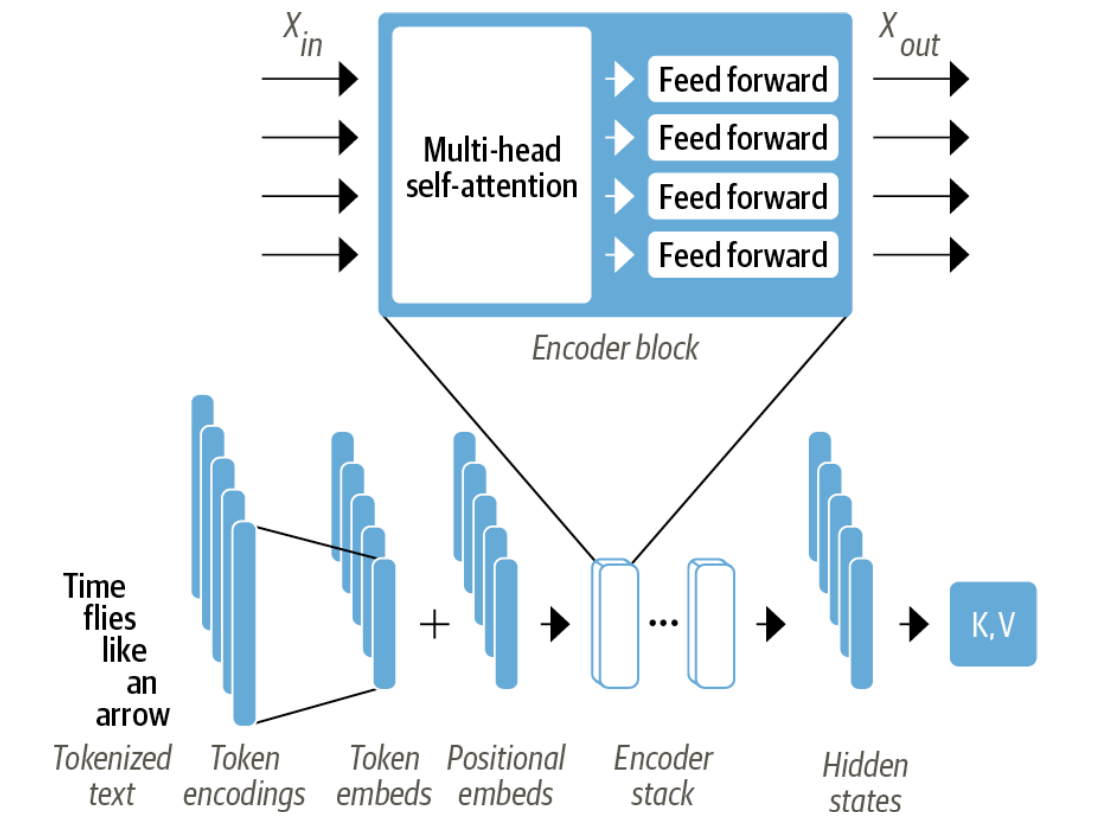
\includegraphics[height=80mm]{graphics/encoder-block.png}
    \caption[Aufbau eines Encoder-Blocks]{Aufbau eines Encoder-Blocks \footnotemark}
    \label{fig:encoder-block}
\end{figure}
\footnotetext{Entnommen aus: \cite{tunstall_natural_2022}, S.60}
%TODO: Complete Chapter: Decoder, Zusammenspiel, Bottleneck -> Relevanz Attention


\chapter{Methodik}
Das folgende Kapitel hat es zum Ziel, den experimentellen Ansatz und die Methodik dieser Arbeit zu beschreiben. Es soll deutlich werden, wie die Forschungsfrage beantwortet wird und welche Schritte dafür notwendig sind. Zunächst werden die zu untersuchenden Modelle aufgelistet. Folgend wird die Anwendung der Forschungsmethode und die entsprechenden Metriken erklärt. Anschließend werden der Aufbau der Testumgebung und die verwendeten Datensätze beschrieben. 
\section{Auswahl der zu untersuchenden Modelle}
Zunächst gilt es die zu untersuchenden Modelle auszuwählen. Die Auswahl der Modelle erfolgt auf Basis der Forschungsfrage und der Zielsetzung dieser Arbeit. Es sollen Modelle untersucht werden, die im Bereich des \ac{VDU} eingesetzt werden können. Die Modelle sollen in der Lage sein, visuelle und textuelle Elemente in Dokumenten zu interpretieren. 

\textbf{Donut:} Das zentrale Modell dieser Arbeit ist \ac{Donut}, gegen welches die OCR-basierten Modelle als Vergleichs- bzw. Referenzmodelle herangezogen werden. Diese Herangehensweise ermöglicht es, die Stärken, Schwächen und Besonderheiten von Donut im Vergleich zu alternativen Methoden des \ac{VDU} zu identifizieren. Es gibt zwar jüngere Nachfolger von \ac{Donut}, jedoch wird in dieser Arbeit ausschließlich Donut untersucht, da es das erste Modell seiner Art ist und die Grundlage für die nachfolgenden Modelle bildet. Es ist in dieser Hinsicht schon etablierter als bspw. \ac{DUBLIN}. Ferner gibt es bereits mehr Forschungsergebnisse zu \ac{Donut} als zu jüngeren Modellen und die Verfügbarkeit von Open-Source Implementierungen ist gegeben.

\textbf{BERT:} \ac{BERT} ist ein rein textbasiertes Modell, welches in der natürlichen Sprachverarbeitung eingesetzt wird. In der Literatur wird es im Bereich des \ac{VDU} einer OCR häufig nachgelagert, um Ergebnisse zu verbessern. \footcites[Vgl. dazu ausführlich][]{nguyen_neural_2020}[Vgl. dazu ausführlich][]{jiang_evaluating_2021} Noch heute wird \ac{BERT} in vielen Forschungen als Vergleichsmodell herangezogen. Eine Eigenschaft, die jedoch beachtet werden muss, ist, dass \ac{BERT} nicht in der Lage ist, visuelle Elemente zu interpretieren. Es handelt sich lediglich um einen Encoder-basierten Transformer, der um keine layoutbasierten Informationen angereichert wurde, \footcites[Vgl. dazu ausführlich][]{devlin_bert_2018} anders als bspw. LayoutLMv3. Es werden in dieser Arbeit die Ergebnisse von \ac{BERT} zu \ac{Donut} im Rahmen der Namend Entity Recognition und der Informationsextraktion verglichen.

%TODO: Fußnote für die Lizenzbedingung anpassen
\textbf{LayoutLMv3:} LayoutLMv3 ist ein performantes und etabliertes OCR-abhängiges Modell. LayoutLM wurde stetig optimiert, bis es Version 3 erreichte. Im FUNSD-Benchmark schneidet es deutlich besser ab als Donut und auch im CORD-Benchmark sind die Ergebnisse besser. \footcites[Vgl. dazu ausführlich][]{huang_layoutlmv3_2022} Der Source-Code von LayoutLMv3 ist zwar einsehbar, jedoch ist das Modell nicht Open-Source. LayoutLMv3 unterliegt strengen Lizenzbedingungen\footcites[Vgl.][]{noauthor_microsoftlayoutlmv3-base_2023} und darf nur für nicht-kommerzielle Zwecke wie Forschung verwendet werden. Daher impliziert der Vergleich von LayoutLMv3 zu Donut mehrere Punkte. Zum einen wird eine Implikation hinsichtlich der Gegenüberstellung von Open-Source und proprietären Modellen gezogen. Zum anderen wird untersucht, ob die proprietäre Implementierung von LayoutLMv3 einen Vorteil gegenüber Donut bringt. Nicht zuletzt wird untersucht, wie OCR-freie Modelle gegenüber OCR-abhängigen Modellen in einer heterogenen, produktionsähnlichen Landschaft an Daten abschneiden.

\section{Metriken des Experiments}
Zuzüglich zu den Modellen, die untersucht werden, ist es notwendig, die Leistungsfähigkeit der Modelle anhand von Metriken zu bewerten. Die Metriken sollen die Effizienz und Genauigkeit der Modelle messen. Sie sollen es ermöglichen, die Modelle miteinander zu vergleichen und die Forschungsfrage bzw. die noch folgenden Hypothesen zu beantworten. Die Metriken, die in dieser Arbeit verwendet werden, sind: Accuracy, F1-Score und \ac{GPUh}. In den folgenden Passagen werden die Metriken und ihre Bedeutung erläutert. Zunächst ist es wichtig, die grundlegende Terminologie zu erläutern, um anschließend die jeweiligen Metriken unter Zunahme der Terminologie erklären zu können. Die Bezeichnungen \emph{positive Klasse} und \emph{negative Klasse} beziehen sich auf die Klassen, wie sie in einer Konfusionsmatrix definiert sind. Die positive Klasse ist die Klasse, die identifiziert werden soll, die negative Klasse ist die Klasse, die nicht identifiziert werden soll. In dieser Arbeit beschreibt \ac{TP} eine Information, die extrahiert wurde und tatsächlich im Dokument vorhanden ist. Ein \ac{TN} liegt vor, wenn eine bestimmte Information oder Entität, wie beispielsweise die Rechnungsnummer, im Dokument nicht vorhanden ist und vom Modell auch nicht extrahiert wurde. Ein \ac{FP} tritt auf, wenn das Modell eine Information oder Entität fälschlicherweise extrahiert, die tatsächlich nicht im Dokument vorhanden ist, oder wenn es eine Information falsch zuordnet, wie zum Beispiel die Fehlinterpretation einer IBAN als Rechnungsnummer. Ein \ac{FN} beschreibt eine Situation, in der eine im Dokument vorhandene und relevante Information, wie die Rechnungsnummer, vom Modell nicht erkannt oder extrahiert wurde. Diese Kategorisierung hilft, die Genauigkeit der Entitätsextraktion zu bewerten, indem sie nicht nur das Vorhandensein, sondern auch die korrekte Identifikation und Zuordnung der Entitäten berücksichtigt.\footcites[Vgl.][]{pawan_confusion_2019}

\textbf{Accuracy:} Die Accuracy ist eine Standardmetrik, die den Anteil der korrekt identifizierten Fälle (sowohl positiv als auch negativ) im Verhältnis zur Gesamtzahl aller Fälle misst. Sie bietet einen schnellen Überblick über die Effektivität eines Modells. Allerdings kann sie in Situationen mit ungleichen Klassenverteilungen irreführend sein, da sie die Effektivität in den einzelnen Klassen nicht differenziert betrachtet. Zusammen mit allen weiteren Metriken befinden sich die Werte zwischen 0 und 1. Ein hoher Wert für die Accuracy zeigt an, dass ein großer Anteil der gesamten Vorhersagen des Modells korrekt ist, sowohl positive als auch negative Vorhersagen. Sie ist besonders aussagekräftig, wenn die Klassen im Datensatz ausgewogen sind.
Ein niedriger Wert für die Accuracy deutet darauf hin, dass das Modell viele Fehler macht, was auf Probleme mit der Modellierung, der Datenqualität oder einer Klassenimbalance hindeuten kann.\footcites[Vgl.][S. 508]{naser_error_2023}
\begin{equation}
    {Accuracy} = \frac{TP + TN}{TP + TN + FP + FN} 
\end{equation}


\textbf{F1-Score:} Der F1-Score ist ein harmonisches Mittel aus Präzision und Recall, das heißt, er berücksichtigt sowohl die Fähigkeit des Modells, relevante Informationen korrekt zu identifizieren (Präzision), als auch die Fähigkeit, alle relevanten Informationen zu erfassen (Recall). Ein niedriger F1-Score weist auf eine oder mehrere der folgenden Situationen hin: Das Modell kann relevante Informationen nicht korrekt identifizieren, es kann relevante Informationen nicht vollständig erfassen oder es kann irrelevante Informationen nicht ausschließen. In jedem Fall führt ein niedriger F1-Score zu einer geringeren Genauigkeit der Informationsgewinnung, was wiederum zu einer ineffizienten und ungenauen Dokumentenverarbeitung führt.

\begin{itemize}
    \item Precision (Präzision) misst den Anteil der korrekt identifizierten positiven Fälle im Verhältnis zu allen Fällen, die vom Modell als positiv eingestuft wurden. Eine hohe Precision bedeutet, dass ein hoher Anteil der positiven Vorhersagen des Modells tatsächlich korrekt ist, was bei Aufgaben wichtig ist, bei denen die Kosten für falsch positive Ergebnisse hoch sind.
    Eine niedrige Precision zeigt an, dass viele der als positiv klassifizierten Fälle falsch sind, was in Szenarien, in denen Vertrauen in das Ergebnis entscheidend ist, problematisch sein kann. \footcites[Vgl.][S. 508]{naser_error_2023}
    \begin{equation}
        Precision = \frac{TP}{TP + FP}
    \end{equation}
    \item Recall (Sensitivität) gibt den Anteil der korrekt identifizierten positiven Fälle im Verhältnis zu allen tatsächlich positiven Fällen an. Ein hoher Recall-Wert zeigt, dass das Modell einen großen Anteil der tatsächlich positiven Fälle korrekt erkennt und extrahiert. Dies ist wichtig in Situationen, wo das Übersehen von positiven Fällen schwerwiegende Folgen haben kann. Ein niedriger Recall bedeutet, dass das Modell viele tatsächliche positive Fälle nicht erkennt, was bei kritischen Anwendungen wie medizinischen Diagnosen oder Betrugserkennung zu ernsthaften Problemen führen kann. \footcites[Vgl.][S. 508]{naser_error_2023}
    \begin{equation}
        Recall = \frac{TP}{TP + FN}
    \end{equation}
\end{itemize}

Indem der F1-Score, Precision und Recall vereint, bietet er eine robuste Bewertung der Modellleistung, die sowohl die Vermeidung von Falsch-Positiven als auch die korrekte Identifikation aller positiven Fälle berücksichtigt. Ein hoher F1-Score ist ein Indikator dafür, dass das Modell sowohl eine hohe Precision als auch einen hohen Recall erreicht hat, was auf eine ausgewogene Leistung in Bezug auf die Vermeidung von falsch positiven und das Übersehen von tatsächlich positiven Fällen hindeutet.
Ein niedriger F1-Score zeigt, dass das Modell entweder viele relevante Fälle übersieht oder viele irrelevante Fälle fälschlicherweise als positiv einstuft, was auf eine schlechte Gesamtleistung des Modells hinweist.\footcites[Vgl.][S. 509]{naser_error_2023}
\begin{equation}
    F_{1} = 2 \cdot \frac{Precision \cdot Recall}{Precision + Recall}
\end{equation}

\textbf{GPUh:} \ac{GPUh} beziehen sich auf die Rechenzeit, die für das Feintuning auf GPU-Hardware benötigt wird. Diese Metrik ist besonders relevant, um die Kosten der Modellentwicklung und -anwendung zu bewerten. Sie ist von großer Bedeutung für kleinere Organisationen oder Einzelpersonen, die möglicherweise nicht über die Ressourcen verfügen, um umfangreiche Datensätze für das Training eigener Modelle zu sammeln oder teure GPU-Ressourcen über längere Zeiträume zu nutzen.

\section{Forschungsdesign}
\subsection{Voraussetzungen für das Experiment}
Das Forschungsdesign dieser Arbeit basiert auf einem experimentellen Ansatz, der darauf abzielt, die Performance von KI-Modellen speziell im Bereich der Informationsextraktion aus Dokumenten, zu untersuchen und zu vergleichen. Dabei liegt der Fokus auf der Evaluation des Donut-Modells im Vergleich zu OCR-abhängigen Modellen wie LayoutLMv3 und BERT, insbesondere unter Produktivbedingungen, die über die Rahmenbedingungen standardisierter Benchmark-Datensätze hinausgehen.

In einem Experiment müssen diverse Voraussetzungen erfüllt werden. Das Untersuchungsobjekt sind im Fall dieser Arbeit die zuvor genannten KI-Modelle und deren Performance in der Informationsextraktion aus Dokumenten. Der Beobachter ist der Forscher, der die Modelle trainiert und evaluiert, sowie die Monitoring-Tools, welche für die Beobachtung des Aufwands der Genauigkeit der Modelle zuständig sind. Der Versuchsaufbau gestaltet sich wie folgt: Zunächst werden die Modelle auf den gleichen Trainingsdatensatz trainiert (Finetuning) und anschließend auf einem Testdatensatz evaluiert. Die Ergebnisse werden anhand der zuvor definierten Metriken gemessen und miteinander verglichen. Der Untersuchungsvorgang wird detailliert in Kapitel 4 beschrieben. Das Experiment wird durchgeführt, um diverse Hypothesen zu überprüfen.

Um Störfaktoren zu minimieren werden identische Daten für Training, Validierung und Test genutzt. Die Daten werden entsprechend vorbereitet, um ein Vermischen von Daten zu vermeiden. Zudem wird auf die Konfiguration von Tokenizern und neuronalen Netzen geachtet, um konsistente Embeddings zu generieren.

Die relevanten Variablen für das Experiment lauten wie folgt:
\begin{itemize}
    \item \textbf{Unabhängige Variablen:} Die unabhängigen Variablen sind die Menge der verwendeten Trainingsdaten, die Hyperparameter der Modelle und die Architektur der Modelle
    \item \textbf{Abhängige Variablen:} Die Performance des Modells, gemessen anhand der Metriken Accuracy, F1-Score und GPUh
\end{itemize}

\subsection{Durchführung des Experiments}
Es werden drei Hypothesen überprüft, die sich auf die Leistungsfähigkeit von Donut im Vergleich zu OCR-abhängigen Modellen beziehen. Die Hypothesen lauten wie folgt:
\begin{itemize}
    \item \textbf{Hypothese 1:} Eine höhere Menge an Daten verbessert die Performance der Modelle, wobei eine abflachende oder sogar abfallende Wirkung bei Overfitting zu beobachten ist.
    \item \textbf{Hypothese 2:} Bei heterogenen Daten erzielt Donut bessere Ergebnisse als LayoutLMv3 und BERT.
    \item \textbf{Hypothese 3:} Die Qualität der vorgelagerten OCR beeinflusst die Ergebnisse von LayoutLMv3 und BERT signifikant.
\end{itemize}

Um die Begriffe der Forschungsfrage und der Hypothesen messbar zu machen, wird durch die Auswahl spezifischer Metriken wie F1-Score, Accuracy und \ac{GPUh} eine klare Messbarkeit der Variablen gewährleistet. Aufgrund der Begrenztheit verfügbarer Daten fungiert der vorhandene Datensatz als Stichprobe. Um die Konsistenz zu gewährleisten, bleibt dieser Datensatz für alle Phasen des Experiments gleich. Es wird höchstens getestet, wie die Modelle abschneiden, wenn lediglich ein Teil des Datensatzes genutzt wird. Dieser Teil ist jedoch für alle Modelle gleich. 

Es werden diverse Vorkehrungen getroffen, um die Gütekriterien des Experiments sicherzustellen. Um eine hohe Validität zu gewährleisten, werden etablierte Metriken verwendet, die die Performance der Modelle objektiv messen. Die Erfassung der \ac{GPUh} erfolgt durch Monitoring-Tools, die die Rechenzeit auf GPU-Hardware messen, um Konsistenz zu gewährleisten. Die Reliabilität (Zuverlässigkeit) wird durch die algorithmische Natur des Experiments gewährleistet. Die Ergebnisse werden dadurch reproduzierbar. Die Objektivität wird durch den Einsatz der Pipeline in Tests von verschiedenen unabhängigen Personen gefördert, die auf unterschiedlichen Rechenplattformen, einschließlich eigener Hardware und Cloud-Diensten, durchgeführt werden. Diese systematische Vorgehensweise ermöglicht eine gründliche Überprüfung der Leistungs- und Effizienzmerkmale des Donut-Modells im Vergleich zu anderen Modellen, wobei ein besonderes Augenmerk auf die praktische Anwendbarkeit und Realitätsnähe der Testbedingungen gelegt wird.

\section{Aufbau der Testumgebung}
Die Testumgebung für die Durchführung der Experimente zur Evaluation der Modellperformance ist sorgfältig ausgewählt und konfiguriert, um repräsentative und zuverlässige Ergebnisse zu gewährleisten. Diese Umgebung ist speziell darauf ausgerichtet, die Anforderungen anspruchsvoller KI-Modelle zu erfüllen und gleichzeitig die Bedingungen eines produktiven Einsatzes nachzuahmen.
% TODO: Anhangsnummern einfügen
Die Experimente werden auf einem leistungsfähigen Rechner durchgeführt, dessen Spezifikationen darauf abgestimmt sind, die rechenintensiven Prozesse des Trainings und des Feintunings der KI-Modelle effizient zu bewältigen. Diese umfassen Nvidia GPUs, welche die \ac{CUDA}-Plattform zum beschleunigten Training unterstützen. Die genauen Spezifikationen der GPU und aller weiteren Komponenten der Rechenmaschienen sind in Angang X aufgeführt. Die Spezifikationen der Cloud-Instanzen, die für die Experimente genutzt werden, sind ebenfalls in Anhang X aufgeführt.

Die für die Experimente verwendeten Datensätze stammen aus dem produktiven Umfeld des Unternehmens und unter anderem von Kunden. Um die Vielfalt realer Anwendungsfälle abzubilden, wird besonderer Wert darauf gelegt, dass die Daten heterogen bezüglich Layout und Text sind. Die Heterogenität der Daten soll sicherstellen, dass die Modelle unter realistischen und anspruchsvollen Bedingungen getestet werden.

Aufgrund der begrenzten Verfügbarkeit von annotierten Datensätzen werden die Daten teilweise mithilfe vom Azure Document Intelligence Studio annotiert. Es ist jedoch zu beachten, dass die Qualität der Annotationen eingeschränkt sein kann, was in späteren Kapiteln diskutiert wird. 

%TODO: Den Teil mit Konstantin nochmal besprechen
Um Datenschutzanforderungen gerecht zu werden und die Verwendung von Kundendaten zu ermöglichen, wird ein strenges Verfahren zur Anonymisierung der Daten angewendet. Dieses Verfahren entfernt oder ersetzt alle personenbezogenen Informationen und andere sensible Daten, um die Privatsphäre zu schützen, während die inhaltliche Integrität der Dokumente für die Zwecke des Experiments erhalten bleibt. Beispielsweise würde der Name des Kunden Max Mustermann durch ein Pseydonym wie Alex Müller ersetzt werden. 

Diese sorgfältige Konfiguration der Testumgebung und Auswahl der Datensätze gewährleistet, dass die Experimente unter Bedingungen durchgeführt werden, die die Anforderungen und Herausforderungen eines produktiven Einsatzes der KI-Modelle für die Dokumentenverarbeitung und -verständnis realistisch abbilden.

%%% Ende des eigentlichen Inhalts %%%

% chapter  (end)

%%% Quellenverzeichnisse (keine Anpassung nötig) %%%
\clearpage
\literaturverzeichnis
%%% Ende Quellenverzeichnisse %%%

\clearpage
\clearpage

\thispagestyle{empty}

{\LARGE\textsf{\textbf{Erklärung zur Verwendung generativer KI-Systeme}}\bigskip}

Bei der Erstellung der eingereichten Arbeit habe ich die nachfolgend aufgeführten auf künstlicher Intelligenz (KI) basierten Systeme benutzt:
% HIER EDITIEREN: (Immer mit \item einen neuen Antrag anführen
\begin{enumerate}
  \item
\end{enumerate}

Ich erkläre, dass ich
\begin{itemize}
  \item mich aktiv über die Leistungsfähigkeit und Beschränkungen der oben genannten KI-Systeme informiert habe, \footnote{U. a. gilt es hierbei zu beachten, dass an KI weitergegebene Inhalte ggf. als Trainingsdaten genutzt und wiederverwendet werden. Dies ist insb. für betriebliche Aspekte als kritisch einzustufen.}
  \item die aus den oben angegebenen KI-Systemen direkt oder sinngemäß übernommenen Passagen gekennzeichnet habe, \footnote{In der Fußnote Ihrer Arbeit geben Sie die KI als Quelle an, z.B.: Erzeugt durch Microsoft Copilot am dd.mm.yyyy. Oder: Entnommen aus einem Dialog mit Perplexity vom dd.mm.yyyy. Oder Absatz 2.3 wurde durch ChatGPT sprachlich geglättet.}
  \item überprüft habe, dass die mithilfe der oben genannten KI-Systeme generierten und von mir übernommenen Inhalte faktisch richtig sind, \footnote{Beispiele hierfür sind u.a. die folgenden Arbeitsschritte: Generierung von Ideen, Konzeption der Arbeit, Literatursuche, Literaturanalyse, Literaturverwaltung, Auswahl von Methoden, Datensammlung, Datenanalyse, Generierung von Programmcodes.}
  \item mir bewusst bin, dass ich als Autorin bzw. Autor dieser Arbeit die Verantwortung für die in ihr gemachten Angaben und Aussagen trage.
\end{itemize}

\vspace{1cm}

Die oben genannten KI-Systeme habe ich wie im Folgenden dargestellt eingesetzt:
\begin{center}
  \begin{tabular}{| p{0.25\linewidth} | p{0.2\linewidth} | p{0.5\linewidth} |}
    \hline
    \textbf{Arbeitsschritt in der wissenschaftlichen Arbeit} & \textbf{Eingesetzte(s) KI-System(e)} & \textbf{Beschreibung der Verwendungsweise} \\
    \hline
    % HIER EDITIEREN: (Nächste Zeile beliebig oft kopieren)
                                                             &                                      &                                            \\
    \hline
  \end{tabular}
\end{center}



%%% Erklärung (keine Anpassungen nötig) %%%
% steht ganz am Ende des Dokuments
\cleardoublepage
\clearpage

\thispagestyle{empty}

{\LARGE\textsf{\textbf{Erklärung}}\bigskip}

% \typMeinerArbeit und \themaMeinerArbeit werden in deckblatt.tex definiert
Ich versichere hiermit, dass ich die vorliegende Arbeit mit dem Thema: \emph{\themaMeinerArbeit} selbstständig verfasst und keine anderen als die angegebenen Quellen und Hilfsmittel benutzt habe.
Ich versichere zudem, dass die eingereichte elektronische Fassung mit der gedruckten Fassung übereinstimmt.

\vspace{3cm}

\begin{center}
  \begin{tabular}{ccc}
    (Ort, Datum) & \hspace{0.3\linewidth} & (Unterschrift)
  \end{tabular}
\end{center}
\end{document}
